\documentclass[12pt,a4paper]{article}
\usepackage{fullpage}
\usepackage[margin=1.5cm]{geometry}
\usepackage{amsmath}
\usepackage{subfig}
\usepackage{graphicx}
\usepackage[justification=centering]{caption}
\usepackage{enumitem}
\usepackage{multirow}
\usepackage{listings}

\begin{document}
\title{Convolutional Neural Networks with PyTorch library}
\author{LE Van Linh}
\date{\today}
\maketitle
\begin{abstract}
In this work, we study a new Deep Learning framework, PyTorch. That is a python package that provides two high-level features (Tensor computation and Deep Networks). In this study, we firstly study the components of PyTorch,how to create a Deep Network with PyTorch. Then, we use this framework to create a network model that we had submitted to ICPRS-18. At the beginning of the model, we use one channel images with the size of $96 \times 96$ as the inputs. To compare with different frameworks (Lasagne), in the experiment part, we will compare the losses and time-consuming during training the model.
\end{abstract}
\section{Pytorch}
PyTorch \cite{paszke2017automatic} is a python package that provides two high-level features:
\begin{itemize}
	\item Tensor computation (like numpy) with strong GPU acceleration,
	\item Deep Neural Networks built on a tape-based autodiff system.
\end{itemize}
In the core of library, PyTorch consists of the following packages:
\begin{itemize}
	\item \textbf{torch}: a Tensor library with GPU support
	\item \textbf{torch.autograd}: supports all Tensor operation in torch
	\item \textbf{torch.nn}: a neural networks library. It deeply integrated with autograd.
	\item \textbf{torch.optim}: an optimization package such as SGD, RMSProp, \ldots which are used with \textit{torch.nn} package
	\item \textbf{torch.multiprocessing}: provides the multiprocessing in python.
	\item \textbf{torch.utils}: provides the helper functions such as DataLoader, Trainer, \ldots
	\item \textbf{torch.legacy(.nn/.optim)}: legacy code that has been ported over from torch for backward compatibility reasons
\end{itemize}
Most frameworks such as TensorFlow, Theano, Caffe and CNTK have a static view of the world. One has to build a neural network, and reuse the same structure again and again. Changing the way the network behaves means that one has to start from scratch. 

With PyTorch, they have a unique way of builiding neural networks: using and replaying a tape recoder. They use a technique called Reserse mode auto-differentiation, which allows the user to change the way the network behaves arbitrarily with zero lag or overhead

\section{Create a neural network with PyTorch}

Neural networks can be constructed using \textbf{torch.nn} package. A \textbf{nn.Module} contains layers, method (\textit{forward}) that return the output. Let's define a network with 2 Convolutional layers followed by 2 Maximum Pooling layers and finish with 3 full-connected layers.\\
\begin{lstlisting}
	import torch
	from torch.autograd import Variable
	import torch.nn as nn
	import torch.nn.functional as F
	
	class Net(nn.Module):

	    def __init__(self):
	    	super(Net, self).__init__()
        	# 1 input image channel, 6 output channels, 
        	#  5x5 square convolution kernel
        	self.conv1 = nn.Conv2d(1, 6, 5)
        	self.conv2 = nn.Conv2d(6, 16, 5)
        	# an affine operation: y = Wx + b
        	self.fc1 = nn.Linear(16 * 5 * 5, 120)
        	self.fc2 = nn.Linear(120, 84)
        	self.fc3 = nn.Linear(84, 10)

	    def forward(self, x):
	    	# Max pooling over a (2, 2) window
        	x = F.max_pool2d(F.relu(self.conv1(x)), (2, 2))
        	# If the size is a square,
        	# you can only specify a single number
        	x = F.max_pool2d(F.relu(self.conv2(x)), 2)
        	x = x.view(-1, self.num_flat_features(x))
        	x = F.relu(self.fc1(x))
        	x = F.relu(self.fc2(x))
        	x = self.fc3(x)
        	return x

	    def num_flat_features(self, x):
	    	# all dimensions except the batch dimension
	    	size = x.size()[1:]  
        	num_features = 1
        	for s in size:
            	num_features *= s
        	return num_features

	net = Net()
	print(net)
\end{lstlisting}

In this network, we just need define the \textbf{forward} function, the \textbf{backward} function will automatically defined for us using \textbf{autograd}.
\section{Landmark predicted model}
In ICPRS-18 paper, we have proposed a network to predict the landmarks on pronotum images. It receives an image of $1 \times 256 \times 192$ as the input. The network was constructed from $3$ \textit{``elementary block"} following by $3$ full-connected layers. An elementary block is defined as a sequence of convolution $(C_i)$, pooling $(P_i)$ and dropout $(D_i)$ layers. The parameters for each layers are as below, the list of values follows the order of elementary blocks:
\begin{itemize}[nosep,label=\footnotesize$\bullet$]
	\item CONV layres:
	\begin{itemize}[nosep]
		\item Number of filters: 32, 64 and 128,
		\item Kernel filters size: $(3 \times 3), (2 \times 2)$, and $(2 \times 2)$
		\item Stride values: $1,1,1$
		\item No padding is used for CONV layers
	\end{itemize}
	\item POOL layers:
	\begin{itemize}[nosep]
		\item Kernel filters size: $(2 \times 2), (2 \times 2)$, and $(2 \times 2)$
		\item Stride values: $2,2,2$
		\item No padding is used for CONV layers
	\end{itemize}
	\item DROP layers:
	\begin{itemize}
		\item Propabilities: $0.1, 0.2$ and $0.3$.
	\end{itemize}
\end{itemize}
In the last full-connected layers (FC), the parameters are: FC1
output: $1000$, FC2 output: $1000$, FC3 output: $16$. As usual, a
dropout layer is inserted between FC1 ond FC2 with a probability equal to $0.5$. Fig.\ref{cnnnetwork2} illustrate the order of the layers in the network.

\begin{figure*}[h]
\centering
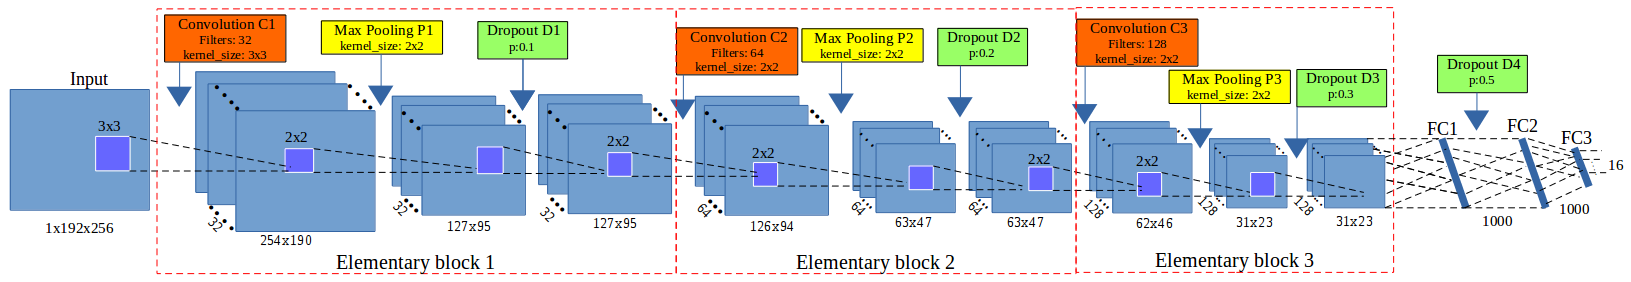
\includegraphics[scale=0.32]{images/cnn_newdatasize/arch_model}
\caption{{\small{Network architecture using $3$ \textit{elementary blocks}.
  Convolution
  layer in red, pooling in yellow and dropout in green color.}}} 
\label{cnnnetwork2}
\end{figure*}

In our study, instead of using a \textit{``square"} image, we have used a \textit{``rectangle"} image as the input. The result shows that the network has the ability to work well on the input that size of width and height are different. Considering as a different of workflows, we would like to see how the network works on ``square" input on another libraries. In this study, we continue to train the proposed network on a new dataset with different size of $96 \times 96$. The network is implemented on PyTorch.

\section{Dataset}
The dataset includes 293 RGB-images of beetle's pronotum. The images were taken by the same camera with the same conditions of resolution of $3264 \times 2448$. The images in the dataset were divided into two subsets: training (including $260$ images) and testing (including $33$ images). For each image, a set of 8 manual landmarks have been set by biologists.
In this section, we introduce the process to down-sample the original images to the new size of images. To obtain the images size of $96 \times 96$, we have applied the procedure following:
\begin{enumerate}[nosep]
	\item Left crop image to obtain the new size of $2448 \times 2448$,
	\item Down-sample the image to size of $96 \times 96$,
	\item Scale the coordinates of the manual landmarks to adapt with the new size of images.
\end{enumerate}

\begin{figure}[h!]
\centering
\subfloat[]{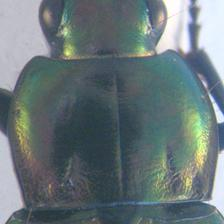
\includegraphics[scale=0.5]{./images/imagenet_finetuning/Prono_001_224}{\label{a2}}}
\caption{An image example in dataset.}
\end{figure}

Then, we augment the images for training and validation (it have been presented in ICPRS-18).

\section{Experiments}
We have trained the model on $2$ different libraries: Lasagne \cite{lasagne} and PyTorch in $10000$ epochs. During training, we have applied differents optimizers (with the same parameters) to compute backprogation. The number of images, which use to train and to validate, are split automatically followed the ratio of $0.8/0.2$. Table.\ref{tab2} shows losses corresponding to the optimizer during training.

\begin{table}[htbp]
\centering
\begin{tabular}{ | p{2cm} | c | c | c | c | c | c | }
\hline
	\multicolumn{1}{|p{2cm}|}{\multirow{2}{*}{Optimizer}} & \multicolumn{3}{c|}{Lasagne} &  \multicolumn{3}{c|}{PyTorch}  \\ \cline{2-7}
	 & Train loss & Validation loss & Time(s) & Train loss & Validation loss & Time(s) \  \\ \hline
	Adam & 0.00011 & 0.00074 & 4,200 & 0.00002 & 0.00286 & 22,500 \\ \hline
	RMSprop & 0.00839 & 0.00778 & 4,308 & 0.00818 & 0.00872 & 23,548 \\ \hline
	SGD Momentum & 0.00041 & 0.00025 & 4,236 & 0.00034 & 0.00154 & 23,264 \\ \hline
	\textbf{SGD Momentum nesterov} & \textbf{0.00015} & \textbf{0.00004} & \textbf{4,258} & \textbf{0.00010} & \textbf{0.00012} & \textbf{24,538} \\ \hline
\end{tabular}
\caption{\small{A comparing of losses during training between the libraries.}}
\label{tab2}
\end{table}
Following Table.\ref{tab2}, we can clearly see the differences between the losses of 2 libraries on the same network with the same data, especially, training time. In the case of \textbf{SGD Momentum nesterov} optimizer, we have obtained the same losses during training model in two libraries.
\section{Conclusions}
In this study, we have studied PyTorch, a new libraries which used to design a Convolutional Neural Network. We have shown the way to create a model with some basic layers. At the end of study, we have trained the model which we have submitted to \textbf{ICPRS-18} in PyTorch. We have trained the model with different optimizers. As the results, mostly the losses are different between two libraries. In which, the large distance between the training times is a worth to consider in the future works.
\bibliographystyle{unsrt}
\bibliography{includes/references}

\end{document}